\subsection{PTZ transform}
	Simply stitching together images will leave us with a large panorama image.
        However, the goal of this project is to emulate pan, tilt and zoom camera motions in post processing, so we must find a way to bring in these motions into our stitching.

	Here we introduce a virtual camera that has the same calibration parameters as the original real cameras.
	With this virtual camera we should be able to look around in the stitched image as a real camera in the real world, but how?
	The motion we seek to describe is in $\mathbb{R}^3$ and the aquired images are in $\mathbb{R}^2$, so we want to describe 3D-dimensional motion, which in this case are camera rotations.
	In order to describe perspective distortions, we introduce a third \emph{homogeneous coordinate}, thereby going from $\mathbb{R}^2$ to $\mathbb{P}^2$.
	The perspective distortion can now be described by a perspective transform matrix, carried out on each pixel in $\mathbb{P}^2$, seen in \cite{hartley2003Multiple}.
	Each pixel, with coordinates $\left( \begin{smallmatrix} x & y & w \end{smallmatrix} \right)^T$
	is multiplied from the left with the transformation matrix, $H_{perspective}$, and the resulting coordinates $ \left( \begin{smallmatrix} x', & y', & w' \end{smallmatrix} \right) ^T$ are the divided with homogeneous coordiante $w$.
	Lastly the pixel coordinates are orthogonally projected down to $\left( \begin{smallmatrix} x'/w', & y'/w' \end{smallmatrix} \right)^T$ and we have returned to $\mathbb{R}^2$, see (\ref{eq:homoapp})

	\begin{multline}
		H_{perspective}\cdot
		\begin{pmatrix}
			x \\
			y \\
			w
		\end{pmatrix}=
		\begin{pmatrix}
			x' \\
			y' \\
			w'
		\end{pmatrix} \rightarrow \\
		\rightarrow
		\begin{pmatrix}
			x' \\
			y' \\
			w'
		\end{pmatrix} \xrightarrow{1/w'}
		\begin{pmatrix}
			x'/w' \\
			y'/w' \\
			1
		\end{pmatrix} \rightarrow
		\begin{pmatrix}
			x'/w' \\
			y'/w'
		\end{pmatrix}
		\label{eq:homoapp}
	\end{multline}

	The perspective transformation matrix, $H_{perspective}$, itself can be decomposed as in (\ref{eq:homodecomp}).
	\begin{equation}
		H_{perspective}=KR_{xyz}K^{-1}
		\label{eq:homodecomp}
	\end{equation}
	where $K$ is a calibration matrix\footnote{which transforms image points from $\mathbb{R}^3$ to $\mathbb{P}^2$} and $R_{xyz}$ is a general rotational matrix in $\mathbb{R}^3$.
$R_{xyz}$ can in turn be decomoposed into $R_x$ (tilt), $R_y$ (pan) and $R_z$, i.e. rotations around the x-, y-, and z-axis of the camera.
The order of these rotations are important as they determine the rotational axi of the camera.
One could think of the rotations all occuring in their own local coordinate systems.
This means that our rotations must occur in the same order as the linkage of the PTZ we want to emulate.
An illustration of the problem can be seen in fig. \ref{fig:PTorTP}.

\begin{figure}[H]
	\centering
	\begin{subfigure}[t]{0.45\columnwidth}
		\centering
		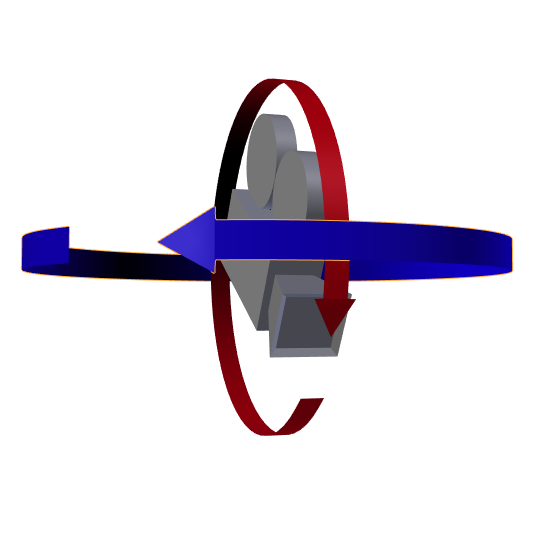
\includegraphics[width=0.8\columnwidth]{../results/images/PanTilt.png}
		\caption{Pan (blue) followed by tilt (red).}
	\end{subfigure}
	\begin{subfigure}[t]{0.45\columnwidth}
		\centering
		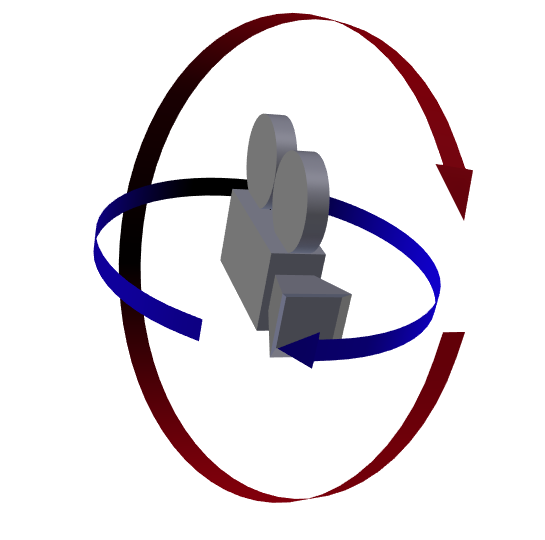
\includegraphics[width=0.8\columnwidth]{../results/images/TiltPan.png}
		\caption{Tilt (red) followed by Pan (blue).}
	\end{subfigure}
	\caption{The rotational axi are depending on the order of the applied rotations}
	\label{fig:PTorTP}
\end{figure}

As many PTZ cameras normally employ a horizontal platform for panning on which the tilting actuators are mounted upon, we therefore first want to apply the pan rotation, (y-direction), and then applying the tilt rotation (x-direction).
However, the input images might have been captured with a tilt in relation to the pan axis.
In this case the initial tilt angle must be estimated first, and the resulting rotation applied prior to to the synthesized pan and tilt rotations.

	For the zooming we scale the images from the cameras point of view, i.e. uniform scalning in the x- and y-direction from the cameras principal point.
	This can be implemented as a scaling matrix of the form in (\ref{eq:zoom}).
	\begin{equation}
		Z=\begin{pmatrix}
			Zoom_x & 0 & 0 \\
			0 & Zoom_y & 0 \\
			0 & 0 & 1
		\end{pmatrix}
		\label{eq:zoom}
	\end{equation}
	where $Zoom_x$ and $Zoom_y$ are scaling factors in the x- and y- direction of the camera.
	It is important that the image origo is placed in the center of the camera in order achive a proper zoom.
	Therefore, we apply the zoom after the rotations in (\ref{eq:homodecomp}). The resulting expression becomes (\ref{eq:finalPTZ})
	\begin{equation}
		H_{perspective}=K Z  R_{x}R_{y}  K^{-1}
		\label{eq:finalPTZ}
	\end{equation}

	We can now accurately describe 3D-rotations as transforms in $\mathbb{P}^2$.

These transforms are applied to all images after the stitching homography, as it is defined for the untransformed images.
